%implementing document formatting:
%page setup (page size, text size, page layout, chapters start on a new page).
%memoir is a form of book class that supports any kind of document.
\documentclass[fleqn,a4paper,12pt,twoside,openany]{memoir}

\usepackage{titlesec}
\usepackage{anysize}
\usepackage{enumitem}

\usepackage{pifont} % extra symbols like (v.. approved)...
\usepackage[hyphens]{url}
\usepackage{array}
\usepackage{multirow}

%\titleformat{\chapter}[display]
%{\normalfont\huge\bfseries}{\chaptertitlename\ \thechapter}{20pt}{\Huge}

% this alters "before" spacing (the second length argument) to 0

\titlespacing*{\chapter}{0pt}{-50pt}{10pt}


%setting the header and footer in that order:
\setheadfoot{28pt}{28pt} %if any problems are encountered, try changing the latter 28pt with 1cm.

%general package syntax: \usepackage[options]{package}

%setting language:
\RequirePackage[danish, english]{babel}

%this package makes it possible to treat any element as a float,
%figures and tables are by default treated as floats.
%read http://en.wikibooks.org/wiki/LaTeX/Floats,_Figures_and_Captions to specify your float.
\usepackage{float}
\usepackage{wrapfig}
\usepackage{placeins}
\usepackage{siunitx}


%this package makes it possible to make theorems and examples:
\usepackage{amsthm}
%setting the style of examples (parameters: plain, definition, remark):
%(definition is usually used for examples)
\theoremstyle{definition}
%the frist parameter is the syntax used in the document, the second is that which is printed in LaTex.
\newtheorem{example}{Example}

%making it possible to use æ, ø and å:
\usepackage[utf8]{inputenc}
%helps with word division when using æ, ø and å, and makes it ps-font rather than bmp:
\usepackage[T1]{fontenc}

%package for implementation of graphic files:
\usepackage{graphicx}

%package for captions
\usepackage[nooneline]{caption}
\captionsetup[table]{name=Tabel}
\usepackage{subcaption}

%%package for implementation of math:
\usepackage{amsmath, amsfonts, amssymb, float, mathtools}

%allowing use of color:
\usepackage[usenames,dvipsnames]{color}
%allowing use of more colors also in tables (see: http://en.wikibooks.org/wiki/LaTeX/Colors):
\usepackage[usenames,dvipsnames,svgnames,table]{xcolor}
\usepackage{colortbl} %Colors for tabulars
\definecolor{pwdrblue}{RGB}{140,140,140} %Color changed back!
\definecolor{darkgrey}{RGB}{180,180,180}
\definecolor{lightgrey}{RGB}{201,201,201}
\definecolor{aaublue}{RGB}{53,46,102}
\definecolor{aausub}{RGB}{154,167,180}
\definecolor{MidnightBlue}{RGB}{25, 25, 112}
\definecolor{NavyBlue}{RGB}{0, 0, 128}
\definecolor{darkgray}{gray}{0.35}
\definecolor{AleeRed}{rgb}{0.5,0,0}
%hyperlinks in the tabel of contents - comment this out before the report is printed.
\usepackage{hyperref}
\hypersetup{
	bookmarks = true,  % Show 'bookmark'-frame in pdf.
	colorlinks = false, % True = colored links, False = framed links.
	citecolor = blue,  % Link color for references.
	linkcolor = blue,  % Link color in table of contents.
	urlcolor = blue,   % Link color for extern URLs.
}

%makes it possible to refer to the name of a chapter rather than just the number.
\usepackage{nameref}
\usepackage[american,cuteinductors,smartlabels]{circuitikz}
\usepackage{tikz}
\usetikzlibrary{shapes,arrows,positioning,calc}
\usetikzlibrary{calc}
\usetikzlibrary{patterns}

%package for writing program code in latex
\usepackage{listings}

\lstset{ 
language=C,               	 	% choose the language of the code
basicstyle=\footnotesize,       % the size of the fonts that are used for the code
numbers=left,                   % where to put the line-numbers
numberstyle=\footnotesize,      % the size of the fonts that are used for the line-numbers
stepnumber=1,                   % the step between two line-numbers. If it is 1 each line will be numbered
numbersep=5pt,                  % how far the line-numbers are from the code
backgroundcolor=\color{white},  % choose the background color. You must add \usepackage{color}
showspaces=false,               % show spaces adding particular underscores
showstringspaces=false,         % underline spaces within strings
showtabs=false,                 % show tabs within strings adding particular underscores
frame=single,           		% adds a frame around the code
tabsize=2,          			% sets default tabsize to 2 spaces
captionpos=b,           		% sets the caption-position to bottom
breaklines=true,       			% sets automatic line breaking
breakatwhitespace=false,    	% sets if automatic breaks should only happen at whitespace
escapeinside={\%*}{*)}          % if you want to add a comment within your code
}

%setting references (using numbers) and supporting i.a. Chicargo-style:

\usepackage{url}

\usepackage[backend=bibtex]{biblatex}
\bibliography{bibliography/bibliography.bib}

\usepackage{verbatim} %enables /begin(comment) and /end{comment} for larger sections

%this package makes it possible include pdf pages in fx appendix;
%using  following syntax: \includepdf[pages={1}]{myfile.pdf}
\usepackage{pdfpages}

\usepackage{pbox} % used for newline in tabular

%%%MARGINER%%%
\setlrmarginsandblock{3.5cm}{2.5cm}{*}	% \setlrmarginsandblock{inner margin}{outer margin}{ratio}
\setulmarginsandblock{2.5cm}{3.0cm}{*}	% \setulmarginsandblock{top}{bottom}{ratio}
\checkandfixthelayout 			            % fixes stuff..

%Enables the use FiXme refferences. Syntax: \fixme{...}
%With "final" in stead of "draft" an error will ocure for every FiXme
%under compilation.
%\usepackage[footnote,draft,english,silent,nomargin]{fixme}

%Centering captions in tables
%\centering
%\captionsetup{justification=centering}
%\caption{bla bla bla}
\usepackage{caption}
\usepackage{pgfplotstable}
\usepackage{pgfplots}

\pgfplotsset{width=15cm,height=7cm}
\usepackage{filecontents}
\usepackage{epstopdf}
\usepackage{nomencl}
\renewcommand{\nomname}{Glossary}
\renewcommand*{\pagedeclaration}[1]{\unskip\dotfill\hyperpage{#1}}
\makenomenclature
\usepackage{makeidx}
\makeindex

%implementing macros:
%%Figure references:
\newcommand{\figref}[1]{\textbf{figur \ref{#1}}}

%Figure references after full stop/period:
\newcommand{\Figref}[1]{\textbf{Figur \ref{#1}}}

%Table references:
\newcommand{\tableref}[1]{\textbf{tabel \ref{#1}}}

%%%CHAPTERLAYOUT%%%
%setting the color of the chapter number
\definecolor{numbercolor}{gray}{0.7}
%Downloaded chapter-setup:
\newif\ifchapternonum
\makechapterstyle{jenor}{
	\setlength{\beforechapskip}{-2cm}	% Adjust space between page top and chapter title.
	\setlength{\afterchapskip}{1.5cm}	% Adjust spave between chapter title and text.
  	\renewcommand\printchaptername{}
  	\renewcommand\printchapternum{}
  	\renewcommand\printchapternonum{\chapternonumtrue}
  	\renewcommand\chaptitlefont{\fontfamily{pbk}\fontseries{db}\fontshape{n}\fontsize{25}{35}\selectfont\raggedleft}
  	\renewcommand\chapnumfont{\fontfamily{pbk}\fontseries{m}\fontshape{n}\fontsize{1in}{0in}\selectfont\color{numbercolor}}
  	\renewcommand\printchaptertitle[1]{%
    \noindent
    \ifchapternonum
    \begin{tabularx}{\textwidth}{X}
    {\let\\\newline\chaptitlefont ##1\par} 
    \end{tabularx}
    \par\vskip-2.5mm\hrule
    \else
    \begin{tabularx}{\textwidth}{Xl}
    {\parbox[b]{\linewidth}{\chaptitlefont ##1}} & \raisebox{-15pt}{\chapnumfont \thechapter}
    \end{tabularx}
    \par\vskip2mm\hrule
    \fi
  }
}
%setting chapter style:
\chapterstyle{jenor}

%depth of numbered headlines (part/chapter/section/subsection):
\setsecnumdepth{subsection}
\maxsecnumdepth{subsection}
%depth of the table of contents:
\settocdepth{section}
\parindent=0pt 

% Makes sure LaTeX does not stretch the text at page break:
\raggedbottom

\newcommand{\img}[4]{
    \begin{figure}[!ht]
    	\centering
    		\includegraphics[width=#4\textwidth]{#1}
    	\caption{\text{#2}}
    	\label{#3}
    \end{figure}
}

\newcommand{\tableimg}[3]{
    \begin{figure}[!ht]
    	\centering
    		\includegraphics[width=#3\textwidth]{#1}
    	\label{#2}
    \end{figure}
}

\newcommand{\wrapimg}[8]{
	\begin{wrapfigure}[10]{#5}{0.4\textwidth} \hspace{0pt}
	\vspace{#6}
  		\begin{center}
   			 \includegraphics[width=#4\textwidth]{#1}
  		\end{center}
  		\vspace{#7}
 		\caption{\textbf{#2}}
 	 	\label{#3}
 	 	\vspace{#8}
	\end{wrapfigure}
}

\newcommand{\sidebyimg}[4]{
	\begin{figure}[H]
		\center
		\begin{subfigure}[b]{0.48\textwidth}
			\includegraphics[width=\textwidth]{#1}
			\caption{#2}
		\end{subfigure}
		\quad
		\begin{subfigure}[b]{0.48\textwidth}
			\includegraphics[width=\textwidth]{#3}
			\caption{#4}
		\end{subfigure}
	\end{figure}
}

\newcommand{\sidebyimglabel}[8]{
	\begin{figure}[H]
		\center
		\begin{subfigure}[b]{0.48\textwidth}
			\includegraphics[width=\textwidth]{#1}
			\caption{#2}
			\label{#3}
		\end{subfigure}
		\quad
		\begin{subfigure}[b]{0.48\textwidth}
			\includegraphics[width=\textwidth]{#4}
			\caption{#5}
			\label{#6}
		\end{subfigure}
		\caption{#7}
		\label{#8}
	\end{figure}
}

\newcommand{\threesidebyimg}[9]{
	\begin{figure}[!htb]
		\minipage{0.32\textwidth}
  			\includegraphics[width=\linewidth]{#1}
  			\caption{\textbf{#2}}\label{fig:#3}
		\endminipage\hfill
		\minipage{0.32\textwidth}
  			\includegraphics[width=\linewidth]{#4}
  			\caption{\textbf{#5}}\label{fig:#6}
		\endminipage\hfill
		\minipage{0.32\textwidth}
  			\includegraphics[width=\linewidth]{#7}
  			\caption{\textbf{#8}}\label{fig:#9}
		\endminipage\hfill
	\threesidebyimgcontinued
}

\newcommand{\threesidebyimgcontinued}[1]{
	\caption{\textbf{#1}}
	\end{figure}
}

\newcommand{\blueheader}[1]{
	\cellcolor{aaublue}\textbf{\color{white}#1}
}
\begin{document}
\nomenclature{UPS}{Uninterruptible power supply}
\nomenclature{CPU}{Central Processing Unit}
\nomenclature{I/O}{Input/Output}
\nomenclature{UPS}{Uninterruptible power supply}
\nomenclature{PCB}{Printed Circuit Board}
\nomenclature{A/C}{Air Condition}
\renewcommand\chaptername{Chapter}
\renewcommand\contentsname{Table of Contents}
\renewcommand\figurename{Figure}
\renewcommand\tablename{Table} 

%implementing front page:
\clearpage
\thispagestyle{empty}

\begin{figure}[H]
	\raggedleft
		
\includegraphics[width=0.2\textwidth]{figures/logo-ucn.png}
\end{figure}
\vspace*{\fill} 
\begin{center}
\begin{Huge}
Vinter Semester 2016\\
\vspace{5 mm}
\textbf{Temperaturænderinger på vandledning}\\
\vspace{3 mm}
Gruppe 1\\
\vspace{3 mm}
1. Semester IT-Teknolog
\end{Huge}
\end{center}

\begin{figure}[h!]
  \centering
  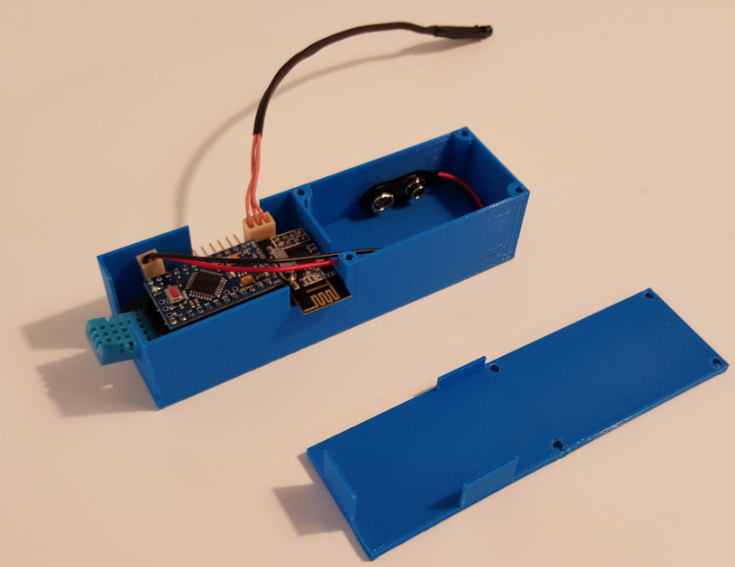
\includegraphics[width=0.7\textwidth]{figures/produkt.png}
\end{figure}

\vspace*{\fill}
\begin{center}
Gruppe medlemmer:
 Anders Pedersen - Benjamin Nielsen - Henrik Jensen - Kasper Delfs - Kristian Porsborg
\end{center}
\begin{center}
Vejledere: Jesper M. Kristensen og Steffen Vutborg
\end{center}
\begin{center}
\line(1,0){400}
\end{center}
%clears one or two pages to make the document start on right hand side:
\cleardoublepage

%numbers the pages with Roman numeral - starts from "i":
\frontmatter

%implementing title sheet:
% Dette er LaTeX-versionen af titelbladet for tek-nat-basis-rapporter 2004 efterår
% Filen kræver:
% Universitetets logo:  aau-logo.png (for LaTeX) eller aau-logo.ps (for LaTeX)
% Synopsis: En fil ved navn synopsis.tex

% Udarbejdet af: Hans Håttel (hans@cs.auc.dk) 21. maj 2003
% Rettet af Morten Christophersen (mortench@tnb.aau.dk) 30. nov 2004(ændret til nyt design 2004 efterår)

%\documentclass[11pt]{article}
%\ifx\pdfoutput\undefined 
%\usepackage[dvips]{graphicx}
%\else
%\usepackage[pdftex]{graphicx} 
%\usepackage{type1cm} \fi
%    \usepackage[ansinew]{inputenc}
%    \usepackage{a4}

%\begin{document} 
\thispagestyle{empty}
%\begin{titlepage}
\begin{nopagebreak}
{\samepage 

\begin{tabular}{r}
\parbox{\textwidth}{  \raisebox{11mm}{
\includegraphics[height=1.5cm]{figures/logo-ucn.png}}
\hfill \hspace{2cm} \parbox{8cm}{\begin{tabular}{l} %4.90
{\small \textbf{\textcolor{MidnightBlue}{1. Semester}}}\\
{\small \textbf{\textcolor{MidnightBlue}{IT-teknolog}}}\\ 
{\small \textcolor{NavyBlue}{Sofiendalsvej 60}} \\
{\small \textcolor{NavyBlue}{9200 Aalborg SV}} \\
{\small \textcolor{NavyBlue}{\emph{http://www.ucn.dk/}}}
\end{tabular}}}
\end{tabular}

\begin{tabular}{cc}
\parbox{7cm}{
\begin{description}

\item { Titel:} 

Temperaturændringer på\\ vandledning

\end{description}

\parbox{8cm}{

\begin{description}
\item { Projekt Periode:}\\
   1. Semester | Vinter semester 2016\\
  \hspace{4cm}
\item { Projectgruppe:}\\
  Gruppe 1 
  \hspace{4cm}
\item { Medvirkende:}\\
Anders Pedersen\\
Benjamin Nielsen\\
Henrik Jensen\\
Kasper Delfs\\
Kristian Porsborg\\
\hspace{2cm}
\item { Vejleder:}\\
Jesper M. Kristensen og \\Steffen Vutborg
  
\end{description}
}
\begin{description}
\item { Sideantal: 26}

\item { Appendiks: 9} 

\item { Færdiggjort: 21/1-2016}
\end{description}
\vfill } &
\parbox{7cm}{
  \vspace{.15cm}
  \hfill 
  \begin{tabular}{l}
   \end{tabular}}
\end{tabular}} \vspace{1.3cm}
\centering
\\
\end{nopagebreak}
%\end{titlepage}
%\end{document}
\chapter*{Forord}

%Læsevejledning:\\
%Kommer senere i projektforløbet.
%\\\\
Dette projekt er udarbejdet af en gruppe 1. semesterstuderende på uddannelsen
IT teknolog på UCN i efteråret 2015. Temaet i projektet er elektroniske systemer.





%
\phantom{Luft}\vspace{3cm}
\begin{table}[H]
	\centering
		\begin{tabular}{c c c}
			\underline{\phantom{JAERJAERJAERJAERGO}} & \phantom{cookies} & \underline{\phantom{JAERJAERJAERJAERGO}} \\
			Anders Pedersen			& \phantom{cookies} & Benjamin Nielsen		\\
			&&\\
			&&\\
			\underline{\phantom{JAERJAERJAERJAERGO}} & \phantom{cookies} & \underline{\phantom{JAERJAERJAERJAERGO}} \\
			Henrik Jensen			& \phantom{cookies} & Kasper Delfs		\\
			&&\\
			&&\\
	    \underline{\phantom{JAERJAERJAERJAERGO}} & \phantom{cookies} & \\
			Kristian Porsborg  					 
			&&\\							
		\end{tabular}
\end{table}

\cleardoublepage

%the '*' allows the tableofcontents be excepted from the actual table of contents.
\tableofcontents*
\newpage
\printnomenclature
\renewcommand*\listfigurename{List of Figures}
\renewcommand*\listtablename{List of Tables}

%numbers the pages with Arabic numeral - starts from 1.
\mainmatter
\chapter{Problemanalyse}
Vandspild er et stort uløst problem, der befinder sig overalt i samfundet. Det koster mange penge hvis et toilet løber eller en vandhane drypper. Derfor har gruppen fået til opgave at udvikle et ikke indgribende produkt, som kan overvåge vandspild hos private og på længere sigt opstille statistikker, som kan hjælpe den private med overvejelser angående renoveringen. Produktet som udvilkes til overvågningen, forbeholes almindelige husstande hvilket medfører et primær fokus på brugervenlighed samt pris.\newline


\section{Bestemmelse af vandtemperatur i rør}
Produktet skal kunne overvåge vandspildet uden at have regulerbare funktioner, dette efterlader muligheden af sammenligningen mellem overflade temperaturen på vandrøret og temperaturen i rummet, endvidere muligheden for at måle fugtigheden.  

\begin{figure}[h!]
  \centering
  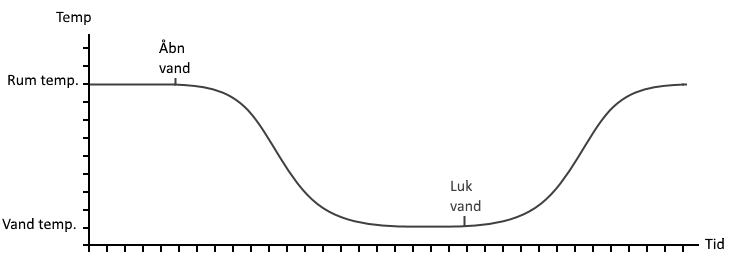
\includegraphics[width=0.7\textwidth]{figures/vandspild_graf_normal.png}
  \caption{Grafen viser overvågningssystemet uden vand spild.}
  \label{vandspild_graf_normal}
\end{figure}



Figur \ref{vandspild_graf_normal} viser hvordan temperaturændringerne forekommer, hvis det antages at der ingen vandspild er og temperaturen på røret derfor er lig med temperaturen i rummet. I det der tilføres nyt vand til huset ændres rørets temperatur og der vil derfor forekomme temperatursvingninger for at kunne aflæse vandspildet.





\begin{figure}[h!]
  \centering
  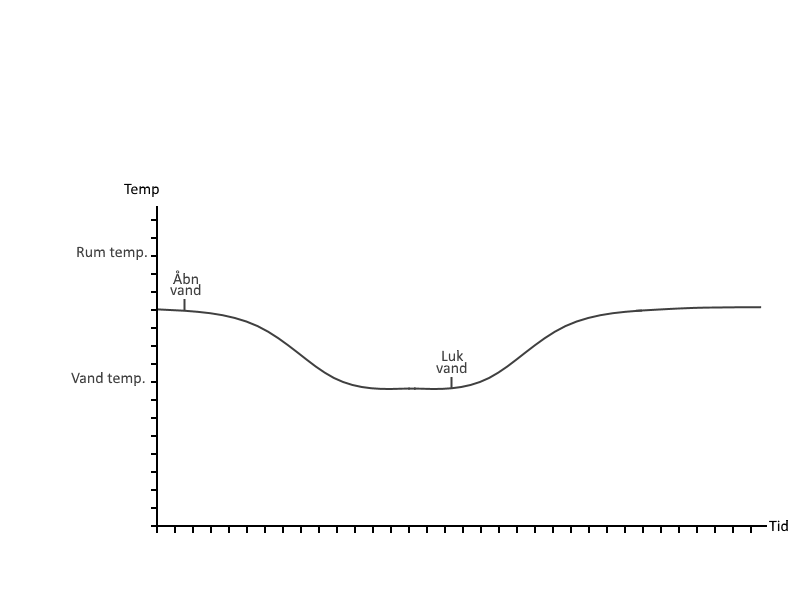
\includegraphics[width=0.7\textwidth]{figures/vandspild_graf_spild.png}
  \caption{Grafen viser overvågningssystemet med vandspild.}
  \label{vandspild_graf_spild}
\end{figure}


Ovenstående figur \ref{vandspild_graf_spild} viser et eksempel på temperaturændringer ved vandspild på et rør. Her ses det hvordan hviletemperaturen på røret aldrig når temperaturen i rummet da vandet aldrig ligger helt stille og derfor tilfører en konstant koldere temperatur.  



    
\chapter{Kravspecifikation}
Det følgende afsnit vil give indblik i de krav, som er opsat for at opfylde de nødvendige kriterier. Fra problemstillingen i projektbeskrivelsen er generelle krav fastlagt og for at imødekomme disse er specifikke krav opsat.  

\hfill \break
Generelle krav
\begin{enumerate}
	\item[•]Produktet kan bygges op omkring et UCN Arduino board. 
	\item[•]Produktet skal bygges med UCN komponenter. Transformer undtaget.
	\item[•]Prototypen skal demonstreres til projekt evalueringen. 
	\item[•]Beregning af pris for produktet samt beregning af udvikling af       produkt.
	\item[•]Projektet skal dokumenteres i form af en rapport.
	\item[•]Produktet skal fungere som en selvstændig enhed.
\end{enumerate}	

Krav til produkt
\begin{enumerate}
	\item[•]Sensor skal benytte 3,3 V eller 5 V da det er kompatibelt med Arduino boardet.
	\item[•]Produktet skal kunne måle temperaturforskelle på rør.
	\item[•]Sensor skal kunne måle temperaturer i mellem 0 og 25$^{\circ}$ C, som bestemmes af temperatursvingninger i vandet.
	\item[•]Præcision på sensor skal være maksimum 1$^{\circ}$ C.
	\item[•]Data skal kunne aflæses i en output terminal.
\end{enumerate}	
	
\chapter{Hardware}
Introduktion til hardware TBD
\section{Hardware krav}
indsæt liste med krav TBD

\section{Hardware struktur og funktionalitet}
Til mikroprocessoren er tilsluttet to sensorer, der hver måler en forskellig temperatur. Den ene er sat direkte på vandledningen, og måler temperaturen på røret, mens den anden sensor sidder så den kan måle temperaturen og luftfugtigheden i rummet - ca. 10 cm fra røret.\newline
Microprocessoren tilspørger sensorerne samtidig og får begge temperaturer samt luftfugtigheden i rummet, og sender disse data til en modtager, en gang hvert 10. sekund.\newline
Serveren eller computeren der modtager data står herefter for udregningen af forskellen på temperaturerne og, ud fra denne, tegning af graf eller visning af data som tekst i terminalen.
\\\\
overbilk og diagram

\begin{figure}[h!]
  \caption{fase1.}
  \centering
  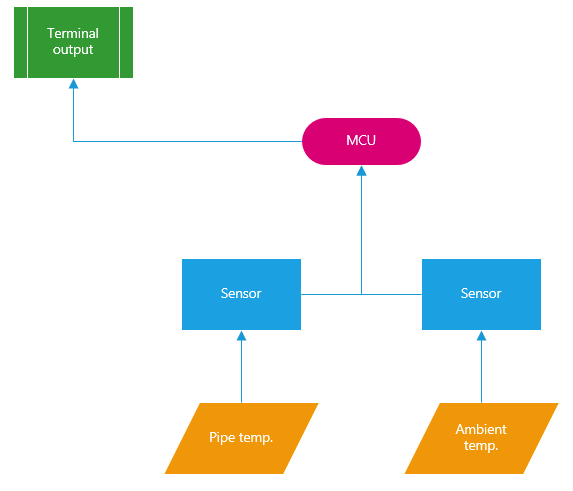
\includegraphics[width=0.5\textwidth]{figures/Phase1.PNG}
\end{figure}


microprocessor (arduino uno)ikke UCN board, da dette ikke indeholder bibliotekerne. TBD

Sensor til subsection TBD



Indsæt undersektioner med de forskellige komponenter TBD

\subsection{Mikroprocessor}

\newpage
\section{Sensor}
Sensoren, som blev beskrevet i hardwareafsnittet, skal kommunikere med Arduino boardet. Dette kræver nogle trin som kan findes i databladet til sensoren. På figur \ref{sensor_min} ses et overblik over funktioner lavet i softwaren, som skal til for at aflæse sensoren. Disse funktioner er konstrueret ud fra databladet, hvor det ses at tre trin skal følges præcist for at tilgå sensoren. De tre trin er en initialisering, ROM command og function command. Herefter er sensoren klar til at blive aflæst.


\begin{figure}[h!]
  \centering
  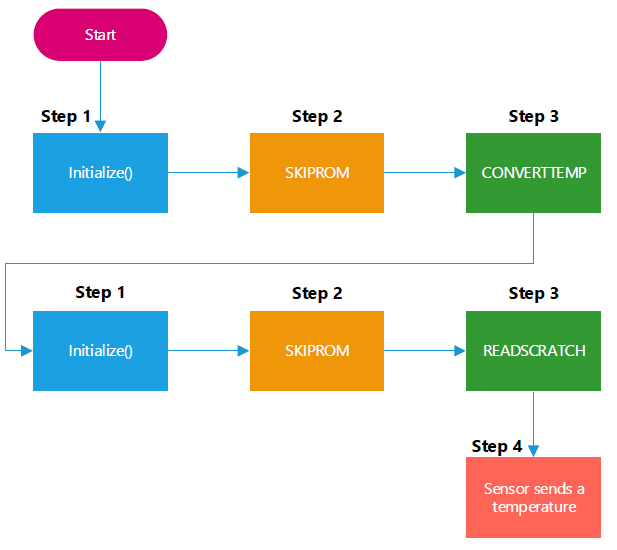
\includegraphics[width=0.9\textwidth]{figures/sensor_minimum.png}
  \caption{Kommunikation med sensor.}
  \label{sensor_min}
\end{figure}

I databladet til DS18B20 sensoren ses et flowchart der viser hvordan mikroprocessoren kommunikerer med sensoren og hvordan den tilgår funktionerne  sensoren kan udføre. Ud fra flowchartet er der konstrueret en mindre version, som indeholder de nødvendige funktioner for at tage en temperaturmåling. Disse funktioner ses på figur \ref{sensor_min}.


\newpage
\subsection{initialize()}
Initialiseringsfunktionen, som ses på flowchartet, er konstrueret ved at finde intervallerne som er nødvendige for at tilgå sensoren over en 1-Wire forbindelse. Disse er aflæst af en graf fra databladet (jf. figur \ref{sensor_min}).
\begin{figure}[h!]
  \centering
  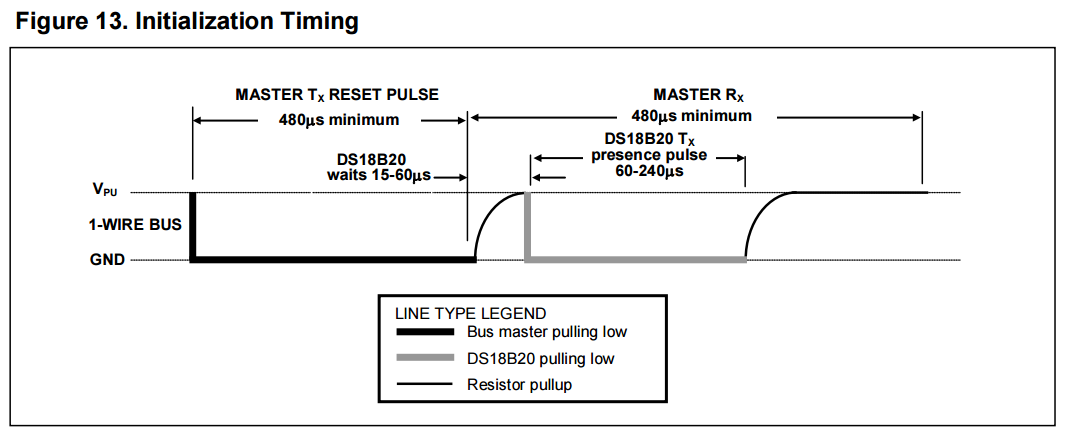
\includegraphics[width=0.9\textwidth]{figures/Initialization_timing.png}
  \caption{Fra datablad om hvordan sensor skal initialiseres.}
  \label{sensor_init}
\end{figure}

Fra databladet ses at 1-Wire forbindelsen skal have en reset pulse i minimum 480$\mu$S og en presence pulse vil herefter blive sendt fra sensoren til mikroprocessoren inden for 60-240$\mu$S. Dette gøres ved at sende et low signal som svarer til reset pulsen. Derefter sættes forbindelsen til input, hvor den vil gå i tri-state mode og pull-up modstanden vil trække signalet højt. 
\\
\\
I koden bliver dette gjort ved at kalde digitalWrite() med low som parameter, i kombination med et delay på 500$\mu$S. Derefter sættes pinMode til input og et delay på 500$\mu$S anvendes igen. Dette kan ses på figur \ref{sensor_kode}.

\begin{figure}[h!]
  \centering
  \fbox{\includegraphics[width=1\textwidth]{figures/Init.png}}
  \caption{Initialisering kode.}
  \label{sensor_kode}
\end{figure}

\subsection{writeByte()}
For at sende kommandoer til sensoren er en writeByte() funktion konstrueret. Den er lavet ud fra samme fremgangsmåde som initialize() funktionen ved at aflæse en graf der indeholder de intervaller der skal til for at tilgå sensoren.

\begin{figure}[h!]
  \centering
  \fbox{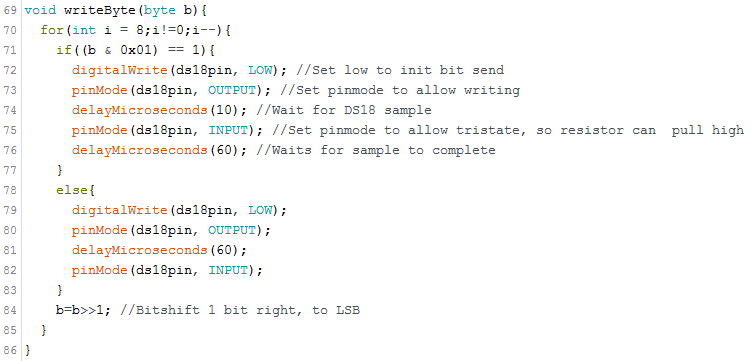
\includegraphics[width=1\textwidth]{figures/write_byte.png}}
  \caption{writeByte() arduino kode.}
  \label{write_byte}
\end{figure}
Det kode som står under if(), er det kode som anvendes hvis der ønskes at skrive et 1 tal og det der står under else(), er det der anvedes til at skrive et 0. Da sensoren modtager 1 bit af gangen, kører for-loopet igennem otte gange . Hver gang en enkelt bit bliver kontrolleret, om der står 1 eller 0, vil der blive foretaget et bitshift til højre og den næste bit vil blive kontrolleret. På denne måde kan der skrives til sensoren.


\subsection{Overblik}

\begin{figure}[h!]
  \centering
  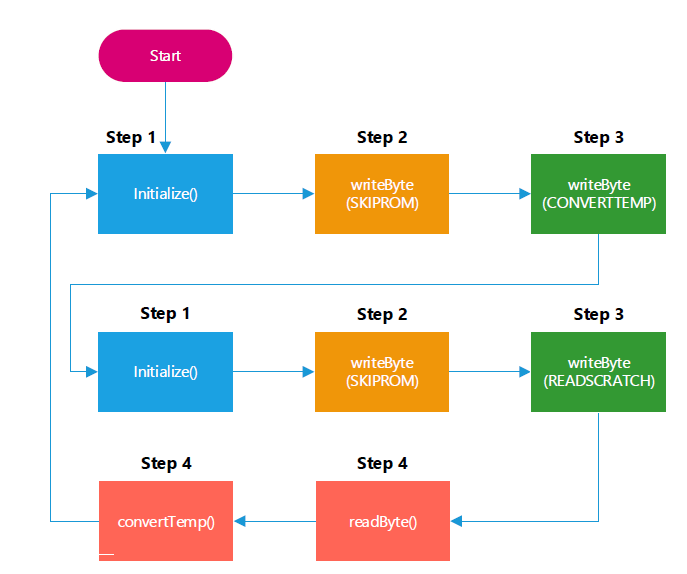
\includegraphics[width=1\textwidth]{figures/sensor_communication.png}
  \caption{De funktioner der skal til for at mikroprocessoren kan kommunikere med sensoren.}
  \label{sensor_total}
\end{figure}
\subsection{Arkitektur}

\begin{figure}[h!]
 \centering
 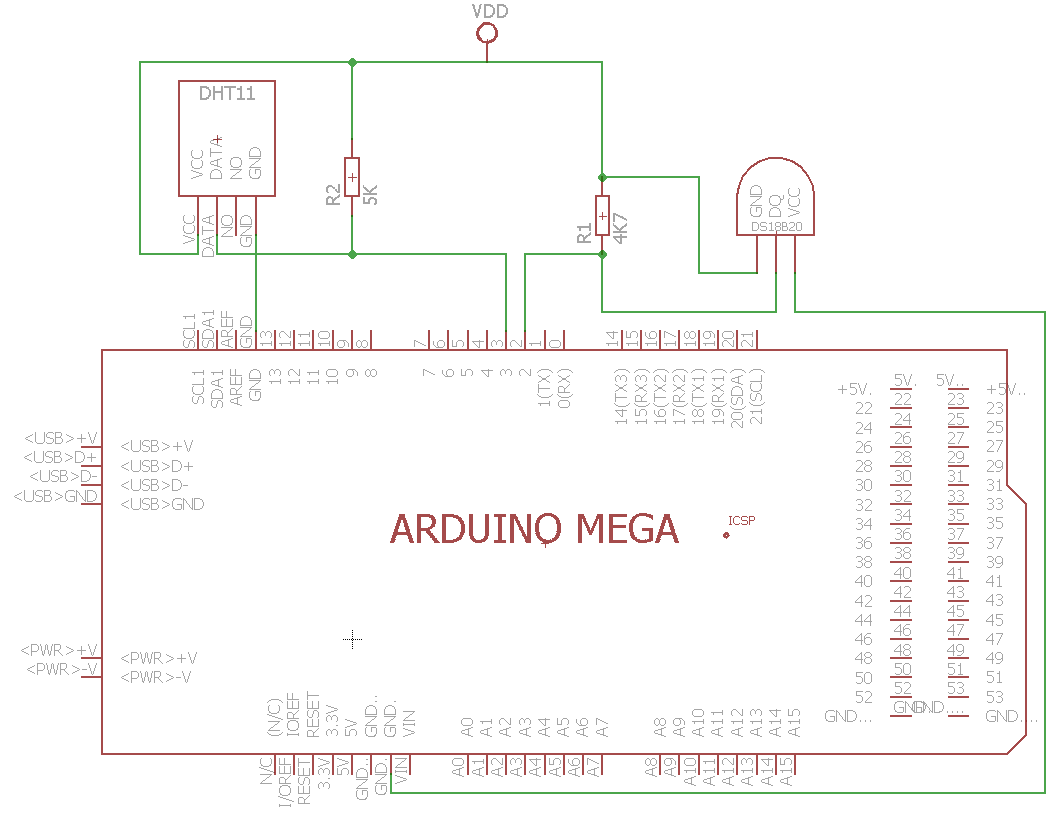
\includegraphics[width=1\textwidth]{figures/phase1_schematic.png}
 \caption{Skematik over mikroprocessor og sensorer.}
 \label{p1_skema}
\end{figure}

Ovenover er vist figur \ref{p1_skema}, som giver et overblik over skemaet af det elektroniske kredsløb brugt til produktet.
Begge sensorer fungerer gennem 1-Wire og deres datalinie er derfor direkte forbundet til mikroprocessoren, og strømtilførslen gennem en modstand.

Til DS18B20 er der valgt at gå væk fra Parasite Power Mode(PPM)\footnote{Sensoren kan modtage strøm gennem datalinien}, da det blev valgt at bruge sensorens egen temperatur konversion, hvilket ville bruge mere strøm end PPM kan tilføre.

\section{Beregning af softwarepris}
Eftersom koden til selve produktet i sig selv ikke fylder så meget, er softwareprisen estimeret til at kræve 35 timer at udvilke samt 15 timer til test, hvilket svarer til ca. 7 arbejdsdage for en enkelt medarbejder.
\begin{table}[h]
\centering
\begin{tabular}{ |p{3cm}||p{3cm}|p{3cm}|p{3cm}|  }
 \hline
 \rowcolor{lightgray}\multicolumn{4}{|c|}{Prisberegning eksl. moms} \\
 \hline
 Software    & pris pr. time &Antal timer&Total\\
 \hline
 Udvikling   & 1000kr    &35&   35000kr\\
 \hline
 Test&   1000kr  & 15   &15000kr\\
 \hline
 		&	&	&\\
 \hline
 Total	&	&	&50000kr\\
 \hline 
\end{tabular}
\caption{Estimeret software pris}
\end{table}


\subsubsection{Samlet pris for produkt}

Den samlede pris for produktet er estimeret til 53442,81kr eksl. moms, fordelt over hardware komponenter og udvkling samt test af software. 

\begin{table}[h]
\centering
\begin{tabular}{ |p{3cm}||p{3cm}|  }
 \hline
 \rowcolor{lightgray}\multicolumn{2}{|c|}{Prisberegning eksl. moms} \\
 \hline
 Hardware    & 3442,81kr \\
 \hline
 Software   & 35000kr   \\
 \hline
  Test&   15000kr   \\
 \hline
 		&\\
 \hline
 Total	&	53442,81kr\\
 \hline 
\end{tabular}
\caption{Samlet produkt pris}
\end{table}

\input{contents/hardware/partconclusion.tex}
\chapter{Software}
\section{Intro}
På figur \ref{initierende_figur} ses den initierende software løsning på problemstillingen.
\begin{figure}[h!]
  \centering
  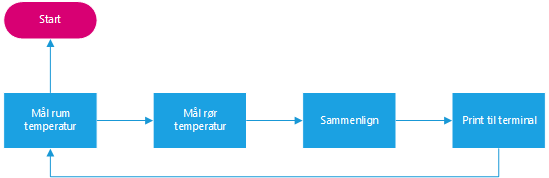
\includegraphics[width=1\textwidth]{figures/Fase1software.png}
  \caption{Initierende software løsning.}
  \label{initierende_figur}
\end{figure}


\section{Specification of the software requirements}
The following section will introduce the necessary requirements for developing the software for a server room surveillance system.\newline
\begin{enumerate}
	\item[•]Intuitively interface.
	\begin{enumerate}
		\item[-]User friendly to reach a broader audience.
	\end{enumerate}
	\item[•]Logging in Intervals of 60 seconds.
	\begin{enumerate}
		\item[-]The reason for measuring data in intervals of 60 seconds is that some readings are close to constant which means there is no need for continuous logging. 
	\end{enumerate}
	\item[•]Dynamic regulation.
	\begin{enumerate}
		\item[-]If the temperature or humidity rises above the predetermined degrees, the A/C will automatically regulate.
	\end{enumerate}
	\item[•]Alarming.
	\begin{enumerate}
		\item[-]If the alarm is triggered, the product needs to inform the server-responsible and technicians.
	\end{enumerate}
\end{enumerate}

\subsection{Software diagram}
\img{figures/softwarediagram.png}{Diagram of the software architecture used.}{softwarediagram}{0.82}
\section{1-Wire protokol}
%https://www.maximintegrated.com/en/products/digital/one-wire.html
Sensoren benytter en 1-Wire forbindelse til at kommunikere med mikroprocessoren. 1-Wire er en teknologi hvor en  enkelt serial forbindelse fungere som data forbindelse i begge retninger. 

Dette gøres ved at forbinde dataforbindelsen på sensoren med mikroprocessoren, og en pull-up modstand forbundes til 5 V som det ses på figur \ref{one_wire_schematic}. 


\begin{figure}[h!]
  \centering
  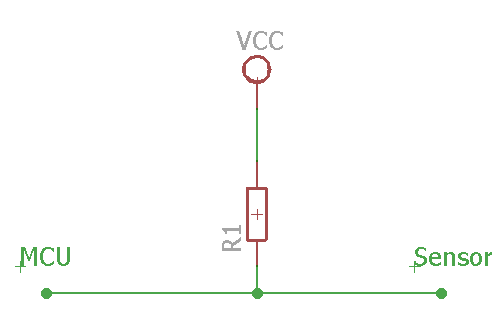
\includegraphics[width=0.8\textwidth]{figures/onewire_eksempel.png}
  \caption{1-Wire data forbindelse mellem sensor og mikroprocessor}
  \label{one_wire_schematic}
\end{figure}

1-wire fungere lidt anderledes end en normal data forbindelse. Data bliver læst som tiden hvor der er et 0 V signal, og pull-op modstanden vil så trække signalet høj hver gang der intet signal er. Der vil ligge 5 V på dataforbindelsen indtil enten sensor eller mikroprocessor begynder at sende 0 V, hvor den anden enhed så kan registrer hvor længe der ligge 0 V på dataforbindelsen. Tidslængden af 0 V signalet afgører om den enheder der modtager skal opfatte signalet som et 0 eller 1. Hvis der skal skrives et 0 udsendes der et 0 V signal i 60 $\mu$S og hvis der skal skrives 1 sendes der 0 V i 15 $\mu$S. 

Når der skal læses over 1-Wire sker dette 30 $\mu$S efter at der er registreret en falded spænding. Dette vil så sige at da 0 svare til et delay på 60 $\mu$S vil der måles 0 V her, og da 1 svare til et delay på maksimum 15 $\mu$S vil der læses 5 V eller et højt signal her.


\begin{figure}[h!]
  \centering
  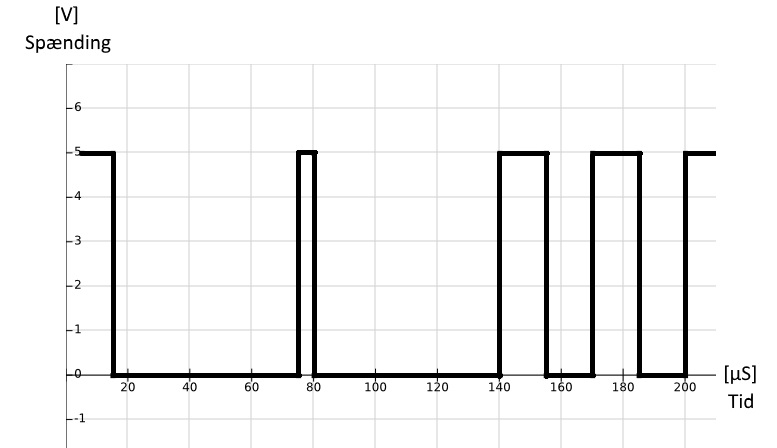
\includegraphics[width=0.8\textwidth]{figures/onewire.png}
  \caption{1-Wire graf der viser hvad der ligger på dataforbindelsen når der bliver skrevet.}
  \label{onewire_graph}
\end{figure}

På figur \ref{onewire_graph} ses det hvordan det vil se ud hvis man ønsker at sende et 0xC over 1-Wire forbindelsen. Det binære tal for 0xC er 1100 og da 1-Wire skriver fra LSB, skal det ses bagfra. Dette ses på grafen som 2 "store" mellemrum hvor der bliver skrevet 0 V på dataforbindelsen efterfuldt af to "korte" som svare til to 1 tal. Dette er blevet eftermålt med et oscilloskop og kan ses på figur \ref{SCR01}.


\begin{figure}[h!]
  \centering
  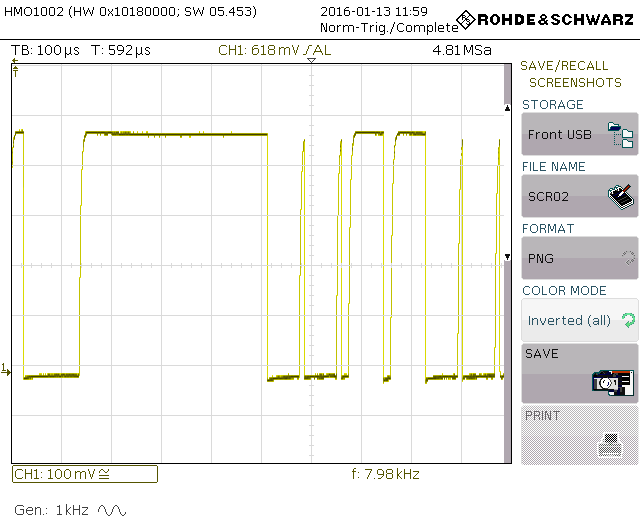
\includegraphics[width=0.8\textwidth]{figures/SCR02.png}
  \caption{Måling af 1-Wire data forbindelse med et oscilloskop.}
  \label{SCR02}
\end{figure}

Figuren viser hvad der måles på dataforbindelsen når mikroprocessoren skriver SKIPROM kommandoen til sensoren.
Fra ca. midten af figuren ses det SKIPROM funktionen som består af 0xCC eller 1100 1100 i binær. Starten af 1100 (læst fra LSB) ses på i midten af grafen.
\newpage
\section{Sensor}
Sensoren, som blev beskrevet i hardwareafsnittet, skal kommunikere med Arduino boardet. Dette kræver nogle trin som kan findes i databladet til sensoren. På figur \ref{sensor_min} ses et overblik over funktioner lavet i softwaren, som skal til for at aflæse sensoren. Disse funktioner er konstrueret ud fra databladet, hvor det ses at tre trin skal følges præcist for at tilgå sensoren. De tre trin er en initialisering, ROM command og function command. Herefter er sensoren klar til at blive aflæst.


\begin{figure}[h!]
  \centering
  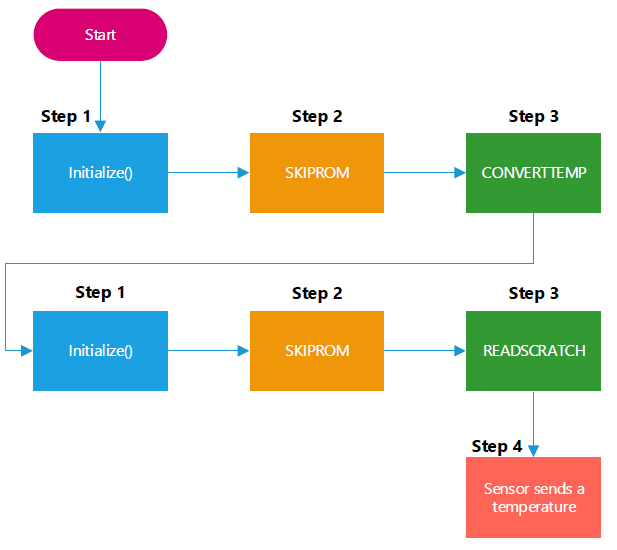
\includegraphics[width=0.9\textwidth]{figures/sensor_minimum.png}
  \caption{Kommunikation med sensor.}
  \label{sensor_min}
\end{figure}

I databladet til DS18B20 sensoren ses et flowchart der viser hvordan mikroprocessoren kommunikerer med sensoren og hvordan den tilgår funktionerne  sensoren kan udføre. Ud fra flowchartet er der konstrueret en mindre version, som indeholder de nødvendige funktioner for at tage en temperaturmåling. Disse funktioner ses på figur \ref{sensor_min}.


\newpage
\subsection{initialize()}
Initialiseringsfunktionen, som ses på flowchartet, er konstrueret ved at finde intervallerne som er nødvendige for at tilgå sensoren over en 1-Wire forbindelse. Disse er aflæst af en graf fra databladet (jf. figur \ref{sensor_min}).
\begin{figure}[h!]
  \centering
  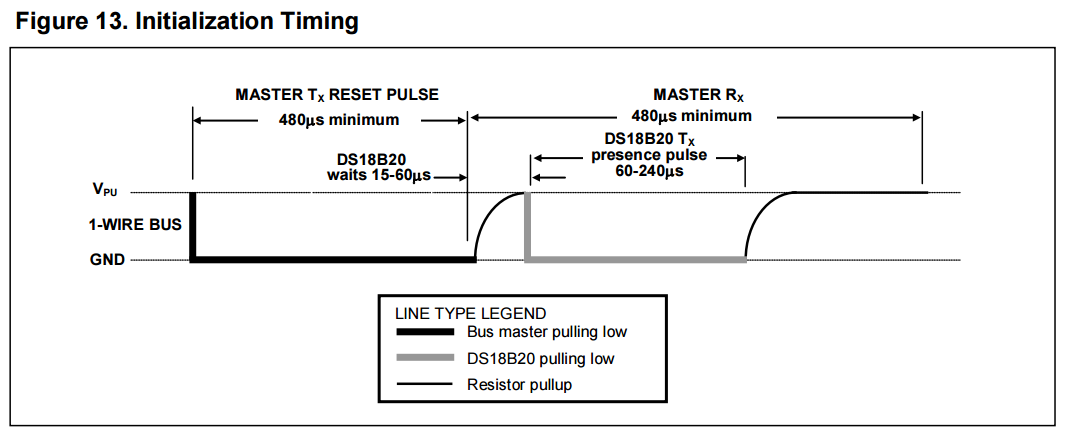
\includegraphics[width=0.9\textwidth]{figures/Initialization_timing.png}
  \caption{Fra datablad om hvordan sensor skal initialiseres.}
  \label{sensor_init}
\end{figure}

Fra databladet ses at 1-Wire forbindelsen skal have en reset pulse i minimum 480$\mu$S og en presence pulse vil herefter blive sendt fra sensoren til mikroprocessoren inden for 60-240$\mu$S. Dette gøres ved at sende et low signal som svarer til reset pulsen. Derefter sættes forbindelsen til input, hvor den vil gå i tri-state mode og pull-up modstanden vil trække signalet højt. 
\\
\\
I koden bliver dette gjort ved at kalde digitalWrite() med low som parameter, i kombination med et delay på 500$\mu$S. Derefter sættes pinMode til input og et delay på 500$\mu$S anvendes igen. Dette kan ses på figur \ref{sensor_kode}.

\begin{figure}[h!]
  \centering
  \fbox{\includegraphics[width=1\textwidth]{figures/Init.png}}
  \caption{Initialisering kode.}
  \label{sensor_kode}
\end{figure}

\subsection{writeByte()}
For at sende kommandoer til sensoren er en writeByte() funktion konstrueret. Den er lavet ud fra samme fremgangsmåde som initialize() funktionen ved at aflæse en graf der indeholder de intervaller der skal til for at tilgå sensoren.

\begin{figure}[h!]
  \centering
  \fbox{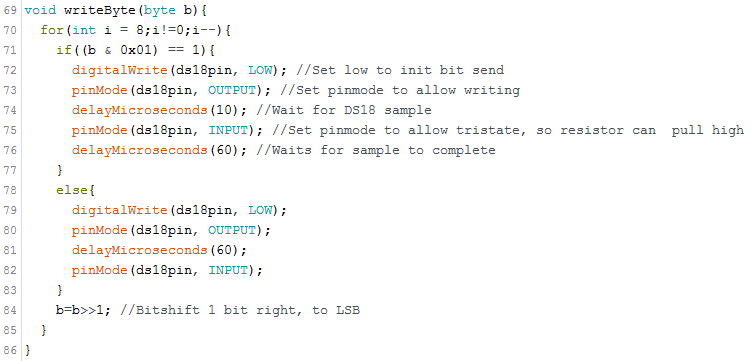
\includegraphics[width=1\textwidth]{figures/write_byte.png}}
  \caption{writeByte() arduino kode.}
  \label{write_byte}
\end{figure}
Det kode som står under if(), er det kode som anvendes hvis der ønskes at skrive et 1 tal og det der står under else(), er det der anvedes til at skrive et 0. Da sensoren modtager 1 bit af gangen, kører for-loopet igennem otte gange . Hver gang en enkelt bit bliver kontrolleret, om der står 1 eller 0, vil der blive foretaget et bitshift til højre og den næste bit vil blive kontrolleret. På denne måde kan der skrives til sensoren.


\subsection{Overblik}

\begin{figure}[h!]
  \centering
  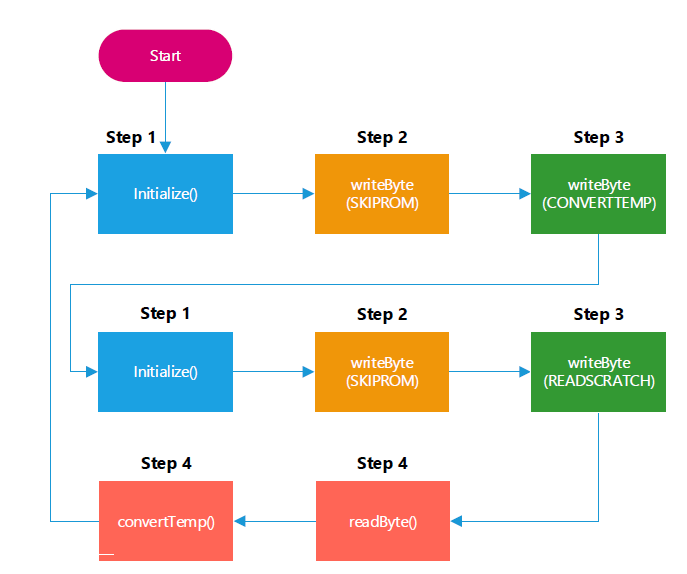
\includegraphics[width=1\textwidth]{figures/sensor_communication.png}
  \caption{De funktioner der skal til for at mikroprocessoren kan kommunikere med sensoren.}
  \label{sensor_total}
\end{figure}
\section{Description of the software structure and functionality}
Based on the previously established requirement specifications and software specifications, a design has been made which is shown in the flowchart above (ref. figure \ref{softwarediagram}). It shows the different pathways, the program is able to take throughout the code with the different functions being shown.

\subsection{Interface}
The product will have two ways to interface it, both a local and a web based interface. The program can be initialized through either of those two interfaces which can be seen on the left side of figure \ref{softwarediagram}. The first thing that happens when the program is initialized is that it performs a self diagnostics. Here it tests if all the sensors are functioning correctly. It is important that the interface is user friendly, so the product is easily accessible by a wide spectrum of users.

\subsection{Main program}
The main program consists of three functions, \textbf{measure, compare} and \textbf{send/save} as seen on figure \ref{mainprogram} below.
\img{figures/mainprogram.png}{Diagram of the main function in the software.}{mainprogram}{0.8}\newline
The main job for the software is to measure the surroundings inside the server room which is done by sensors. These sensors will record values which will be compared to parameters corresponding to safe margins for the different sensors. They can be predefined or set by a user on a later point. Then the recorded values will be stored on a local storage, and sent to an offsite server and stored there as well for extra redundancy in the system.

\subsection{No alarm}
If the measured data in the main program matches the parameters set beforehand by the technicians, no alarm will be given and the program will return to the main program, where it will continue to run the loop.
\img{figures/noalarm.png}{Diagram of no alarm loop.}{noalarm}{0.8}\newline

The green arrows in figure \ref{noalarm}. shows the loop that will be running if there are no measurements outside the given parameters. This loop will be running unless there is an alarm.

\subsection{Alarm}
If the measured data on the sensors does not match the predetermined set of parameters, an alarm will be triggered. This alarm will give notice to the user / admin and the technician via email and text message. The email will contain information about which sensors are above the threshold, so the user and  the technicians know which precautions they need to take.
\newpage
After the program has given notice about the alarm, it will return to the main program, and start measuring the data from the sensors again.\newline
\img{figures/alarmloop.png}{Diagram of loop if there is an alarm.}{alarmloop}{0.8}\newline
\newline
The red arrows in diagram \ref{alarmloop}. shows the loop that will be running if an alarm is necessary. This loop will only be running if any of the measurements is outside the given parameters.

\subsection{Regulate}
If the temperature sensors has readings outside the predetermined parameters, the system itself is able to adjust the A/C. This is a precaution the system has to be able to run if the server room gets a temperature that's higher than the predetermined values.\clearpage
\img{figures/regulateloop.png}{Diagram of the loop when the program regulates the A/C.}{regulateloop}{0.8}
Figure \ref{regulateloop} show the loop the program normally will be running when the sensors log a temperature that does not match the parameters. As shown by the blue arrows in the diagram \ref{regulateloop}, the program checks the values and if they do not match the given parameters, it will regulate the A/C. The program will then use the same loop as if no alarm.
\newline
In some circumstances the program will need to give an alarm and thereby deviate from the loop that normally runs.  This loop sequence will only be initialized, when the program has tried to regulate the A/C for a predetermined amount of time without getting the temperature to fit the predetermined values.  This is determined by the size of the room in order to specify how long it takes to apply the regulation.
\section{Beregning af softwarepris}
Eftersom koden til selve produktet i sig selv ikke fylder så meget, er softwareprisen estimeret til at kræve 35 timer at udvilke samt 15 timer til test, hvilket svarer til ca. 7 arbejdsdage for en enkelt medarbejder.
\begin{table}[h]
\centering
\begin{tabular}{ |p{3cm}||p{3cm}|p{3cm}|p{3cm}|  }
 \hline
 \rowcolor{lightgray}\multicolumn{4}{|c|}{Prisberegning eksl. moms} \\
 \hline
 Software    & pris pr. time &Antal timer&Total\\
 \hline
 Udvikling   & 1000kr    &35&   35000kr\\
 \hline
 Test&   1000kr  & 15   &15000kr\\
 \hline
 		&	&	&\\
 \hline
 Total	&	&	&50000kr\\
 \hline 
\end{tabular}
\caption{Estimeret software pris}
\end{table}


\subsubsection{Samlet pris for produkt}

Den samlede pris for produktet er estimeret til 53442,81kr eksl. moms, fordelt over hardware komponenter og udvkling samt test af software. 

\begin{table}[h]
\centering
\begin{tabular}{ |p{3cm}||p{3cm}|  }
 \hline
 \rowcolor{lightgray}\multicolumn{2}{|c|}{Prisberegning eksl. moms} \\
 \hline
 Hardware    & 3442,81kr \\
 \hline
 Software   & 35000kr   \\
 \hline
  Test&   15000kr   \\
 \hline
 		&\\
 \hline
 Total	&	53442,81kr\\
 \hline 
\end{tabular}
\caption{Samlet produkt pris}
\end{table}

\input{contents/software/partconclusion.tex}
\chapter{Accepttest}
\fxnote{ beskriv accepttest og diskuter}
\chapter{Videre udvikling}
Som et led i arbejd processen med udvikling af systemet er der blevet arbejdet på hvordan det system kan videre udvikles til at have mere funktion i forhold til at dette system skulle anvendes i en virkeligheds situation.

\section{Data logning}
Den første del af videre udviklingen består i at gøre systemet i stand til ikke bare at kunne visse de målte data og anden beregning der bliver foretaget, men at logge det over tid så det både kan bruges til at logfører markante ændringer over tid, samt at kunne fremvise det loggede data for en forbruger af systemet.

\subsection{Arduino [Hello world]\fixme{mangler bedre titel}}
For at gøre systemet i stand til at kunne logge de målte og beregnede data er der til dette projekt blevet valgt at bruge et Arduino Ethernet Shield for at finde arduinoen med internettet, samt der er blevet skrevet kode der gør det muligt for arduinoen at lægge data op på en SQL database på nettet.
\img{figures/ethernetshield.jpg}{Arduino Ethernet Shield. Foto af: http://tech-things.net/}{ethernetshield}{0.7}\newline
program flowet med brugen af ethernet shieldet følger det samme flow vist i figur \ref{fase1flow}
med undtagelse af det sidste led værende "Print til terminal", i stedet bliver der nu oprettet en forbindelse til en PHP side på nettet hvor efter arduinoen sender en HTTP POST pakke til siden, derved ser det nye flow således sådan ud:
\img{figures/fase2software2.png}{Ethernet flowchart}{ethernetflowchart}{0.8}\newline
Efter POST pakken er blevet sendt bliver den læst af PHP siden som derefter splitter pakken i de individuelle data punkter som er:
\begin{enumerate}
	\item[•]Node ID
	\item[•]Rør temperatur
	\item[•]Rum temperatur
	\item[•]Rum luft fugtighed
\end{enumerate}
Som det sidste forbinder PHP siden så til en SQL database og sender dataen op til den og lukker forbindelsen.
\begin{figure}[!ht]
	\begin{lstlisting}
<?php
include("../includes/config.php");
$sql = $con->prepare("INSERT INTO data(node_unit, node_pipetemp, node_hum, node_ambitemp, node_time)VALUES(?, ?, ?, ?, ?)");
$sql->bind_param("sssss", $node_unit, $node_pipetemp, $node_hum, $node_ambitemp, $node_time);

$node_data = $_GET['data'];
$node_dataArray = explode(',', $node_data);

$node_unit = $node_dataArray[0];
$node_pipetemp = $node_dataArray[1];
$node_hum = $node_dataArray[3];
$node_ambitemp = $node_dataArray[2];
date_default_timezone_set("Europe/Copenhagen"); 
$node_time = time(); 
$sql->execute();
$sql->close();
?>
\end{lstlisting}
\caption{PHP kode til SQL logning}
\label{phpsql}
\end{figure}

\subsection{GUI hjemmeside}
Med tilføjelsen af SQL datalogning har det givet nem adgang til at kunne illustrerer det loggede data til forbrugeren af systemet.
Der er som en del af videre udviklingen blevet lavet et simpelt interface bestående af en hjemmeside som er programmeret i en blanding af sprogende PHP og javascript samt HTML.
\img{figures/webguimain.png}{Hovedsiden af bruger interfacet\fixme{opdatere billedet med ds18 data}}{webguimain}{1}\newline
Ideen med hjemmesiden er at gøre det nemt for forbrugeren at monitorer hvordan det forløber med det data der kommer ind fra de enheder der er forbundet til den, samt at det er i stand til at kunne vise hvis der skulle være beskeder fra systemet.

\section{Lejligheds løsning}
Som det sidste led i videre udviklings processen er der blevet kigget på hvordan system kan blive videre bygget til at kunne fungere som en samlet enheds i et lejligheds kompleks. For at gøre systemet mere flexibelt og modulært er der blevet fokuseret på at forbinde måleenheder men en master enhed via radio moduler. målenhederne snakket med hinanden og masteren intern over radio enhederne og master modtager det målte data fra måleenhederne og sender det op til SQL serveren til logning.

\subsection{Radio moduler}
Til den interne kommunikation mellem målenhederne er der i dette projekt blevet valgt at bruge radio modulet NRF04L01+ fra Nordic Semiconductors.
\img{figures/nrf24l01.png}{NRF24L01+ Radio modul}{nrf24l01}{0.2}\newline
Dette er en lille og meget billig radio modul som kommunikere med en båndbredde på 2.4GHz men benytter sig som standard af UDP og TCP protokoller som f.eks WiFi gør. 
Kommnukationen mellem mikrocontrolleren sker via en seriel SPI forbindelse og gør at det er muligt at bruge modulet på næsten alle mikrocontrollere der findes.

\subsection{Mesh netværk}
\subsubsection*{P2P}
Radio modulet kan sættes op til at kommunikere på flere forskellige måder afhængigt af hvad der er behov for i den anvendte situation.
Den første og mest anvendte metode er P2P (Point 2 Point).
\img{figures/p2p.png}{Point 2 point diagram}{p2pdiagram}{0.4}\newline
P2P er en effektiv forbindelses konfiguration hvis man skal have to enheder til at snakke sammen individuelt med en simpel forbindelse. Denne løsning ville være brugbar til projektet hvis der kun var tale om en måleenhed og en master der skulle kommunikere trådløst, dette er dog langt fra ideelt til en flexibel løsning som det ønskes at anvende disse radio moduler til hvor der er flere en 1 måleenhed.

\subsubsection*{Stjerne netværk}
Den næste mulige netværk konfiguration er er bedst kendt som et stjerne netværk. denne type netværk er en viderebygning af tidligere nævnte P2P model, da man her, i stedet for kun har to enheder der kan kommunikere med hinanden, har en master enhed der kan kommunikere med mange enheder på engang. Dette er en klar fordel da man nu i forhold til at, skulle det anvendes til lejlighedsløsningen, har mulighed for at have så mange enheder der er brug for som så kan måle de data punkter de skal, for at så derved at kunne sende det til masteren som så kan sende det videre.
\img{figures/starnetwork.png}{Star netværks diagram}{starnetworkdiagram}{0.6}\newline
Begrænsningen ved at anvende et stjerne netværk til lejlighedsløsningen ligger i at alle enheder skal kunne have radio forbindelse til masteren, hvilket kan være en meget stor udfordring i lejligheds komplekser, da der her er mange vægge og andre signal forstyrrende elementer signalet skal vandre igennem for at nå masteren.

\subsubsection*{Mesh netværk}
Signal problemet som opstår ved at anvende et stjerne netværk kan løses ved at anvende en netværks type bedst kendet som et mesh netværk.
Et mest netværk er på nogle måder en videreudvikling at stjerne netværk, hvor man nu, i stedet for kun at have en master der kan snakke med alle enheder, har enheder som kan fungere som mellemstationer mellem de yderste noder og masteren \ref{meshnetworkdiagram}
\img{figures/meshnetwork.png}{Mesh netværks diagram}{meshnetworkdiagram}{1}
\chapter{Konklusion}
\section{konklusion}
%Opgavebeskrivelse
I denne opgave var formålet at designe, implementere og teste et elektronisk system med henblik på overvågning af vandspild i private husstande.
\\ 
\\
%Overblik
Løsningen er designet omkring et Arduino board, en ds18b20 sensor til måling af temperatur på røret og en dht11 sensor til måling af temperatur og fugtighed i  rummet.
\\
\\
%Fremgangsmåde
Gruppen har ved hjælp af et Arduino board og to sensorer implementeret et software, som blev bygget fra bunden. Softwaren kan deles op i tre dele, et bibliotek til anvendelse af sensor ds18b20 som blev skrevet ud fra det tilhørende datablad, sensor dht11  og et hovedprogram til styring af funktioner            
%Videreudvikling

\chapter{Appendiks}
\section{Gruppekontrakt}
\subsection{Kontaktinformation}
\begin{table}[h]
\centering

\begin{tabular}{|l|l|l|p{4cm}|}
\hline
\rowcolor{lightgray}
Navn			  & E-mail					 & Telefon     & Adresse 							 \\ \hline
Anders Pedersen   & andped13@gmail.com       & 42 55 12 59 & Brandevej 10, 129220 Aalborg Øst    \\ \hline
Benjamin Nielsen  & yipiyuk5@gmail.com       & 30 42 76 45 & Årestrupsvej 32, 2. tv 9000 Aalborg \\ \hline
Henrik Jensen     & Barista.desner@gmail.com & 28 56 89 34 & Myrdalstræde 158, 9220 Aalborg Øst  \\ \hline
Kasper Delfs      & kasper.delfs@gmail.com   & 60 62 89 32 & Klintevej 9, 9560 Hadsund           \\ \hline
Kristian Porsborg & Pors\_smith@hotmail.com  & 22 28 95 95 & Prinsensgade 12, 3 tv. 9000 Aalborg \\ \hline
\end{tabular}
\caption{Kontakt information}
\label{kontaktinformation}
\end{table}

\subsection{Arbejdsgang}
Ud fra nedenstående figur vises gruppens arbejdsgang. 

\subsection{Milesten og mål}
\fxnote{Indsæt milesten}

\subsection{Deadline}
\begin{enumerate}
	\item[•]Afleveringsdato: 22. januar kl. 12:00.
\end{enumerate}

\section{User guide}
The following includes a description to set up and install the system.
\img{figures/userGuide.png}{User guide diagram}{userGuideDiagram}{0.8}
\subsection*{Step 1}
\begin{enumerate}
	\item[•]Connect the sensors to the product.
\end{enumerate}
\subsection*{Step 2}
\begin{enumerate}
	\item[•]Connect the product to the ethernet.
\end{enumerate}
\subsection*{Step 3}
\begin{enumerate}
	\item[•]Connect the product to a power source.  
\end{enumerate}
\chapter{Litteraturliste}
\fxnote{færdiggør kildeliste}
\begin{enumerate}
	\item[•] \url{https://ucn.instructure.com/courses/2130/wiki}
	\item[•] \url{https://www.arduino.cc/en/Main/ArduinoBoardUno}
	\item[•] \url{https://www.arduino.cc/en/Main/ArduinoBoardProMini}
	\item[•] \url{https://www.sparkfun.com/datasheets/Components/SMD/nRF24L01Pluss_Preliminary_Product_Specification_v1_0.pdf}
\end{enumerate}



\newpage
\listoffigures
\addtocontents{lof}{~\hfill\textbf{Page}\par}
\fxnote{indsæt figurliste, eller slet siden helt}
\newpage
\listoftables
\addtocontents{lot}{~\hfill\textbf{Page}\par}
\fxnote{indsæt tabelliste, eller slet siden helt}
\newpage
\printbibliography
\listoffixmes

\end{document}